\documentclass[8pt]{beamer}

\usetheme{Darmstadt}
\usecolortheme{dove}
\usepackage[small,center]{caption}
\usepackage{times}
\usefonttheme{structurebold}
\usepackage[english]{babel}
\usepackage{pgf,pgfarrows,pgfnodes,pgfautomata,pgfheaps}
\usepackage{amsmath,amssymb}
\usepackage{amsxtra}

\usepackage{caption}
\usepackage{tikz}
\usetikzlibrary{shapes.misc}

\newcommand{\leftd}[1]{{\color{red} \bar{#1}}}
\newcommand{\interface}[2]{{\color{blue}{#1}_I(#2)}}
\newcommand{\leftdd}[2]{{\color{red} \bar{#1}(\bar{#2})}}
\newcommand{\leftFourier}[1]{{\color{red} \hat{#1}}}
\newcommand{\leftFourierTwo}[2]{{\color{red} \hat{#1}(\hat{#2})}}
\newcommand{\half}{\dfrac{1}{2}}
\newcommand{\divergence}{\mathrm{div}}

\newcommand{\I}{I}

\newcommand*{\vcenterimage}[1]{\vcenter{\hbox{\includegraphics[width=2in]{#1}}}}
\newcommand*{\vcenterarrow}{\vcenter{\hbox{$\Longrightarrow$}}}

\definecolor{Carolinablue}{RGB}{75, 156, 211}
\definecolor{ballblue}{rgb}{0.13, 0.67, 0.8}
\definecolor{lightgray}{rgb}{0.83, 0.83, 0.83}
\setbeamercolor{block title}{bg=lightgray,fg=Carolinablue}
\setbeamercolor{block body}{bg=white,fg=black}
\setbeamercovered{dynamic}
\setbeamercolor*{item}{fg=Carolinablue}

\DeclareMathOperator{\hyphen}{-}

\captionsetup[subfigure]{labelformat=empty}
\captionsetup[figure]{labelformat=empty}
\setbeamertemplate{navigation symbols}{}
\setbeamertemplate{footline}[frame number]
\begin{document}

% tikz stuff
\tikzset{cross/.style={cross out, draw=black, minimum size=2*(#1-\pgflinewidth),
inner sep=0pt, outer sep=0pt},
%default radius will be 1pt.
cross/.default={2.5pt}}



\frame{
\title{\Large Improving Boundary Derivative Recovery in Elliptic PDEs}

\author{{\Large David Wells \\\vspace{0.1in} University of North Carolina}    \\
\vspace{0.2in} {In collaboration with:\\{}J. W. Banks (RPI)}}

\date{June 4, 2019\\{} North American Higher Order Methods Conference, San Diego}

\begin{figure}[h]
\centering

\includegraphics[width=1.5in]{UNC_logo_542.eps}
 \end{figure}%

\vspace{-0.2in}
\titlepage
}

\section{Goals}
    \begin{frame}
        \frametitle{Goals}
        \begin{itemize}
            \item Efficient numerical methods for elliptic PDEs
            \item Develop new theoretical tools
            \item Increased accuracy in (normal) boundary derivatives
            \item No postprocessing (achieve an energy estimate)
            \item Order \(n + 1\) data should lead to order \(n + 1\) derivatives
        \end{itemize}
    \end{frame}

\section{Superconvergence}
\begin{frame}
    \frametitle{Assumptions}
    \begin{itemize}
        \item Linear, constant coefficient elliptic PDEs, Dirichlet (or
              periodic) boundary conditions
              \pause
        \item \emph{Lots} of regularity
              \pause
        \item Uniform grid (constant \(\Delta x\), \(\Delta y\)) of tensor
              product elements (no triangles)
              \pause
        \item Continuous finite element spaces
              \begin{itemize}
                  \item in 1D, degree \(n\) on interior elements, degree \(n +
                        p\) on nonperiodic edge elements
                  \item in 2D, bilinear on interior elements, degree \(1 \otimes
                        1 + p\) on nonperiodic edge elements
              \end{itemize}
    \end{itemize}
\end{frame}

\begin{frame}
    \frametitle{What's the plan?}
    \begin{itemize}
        \item Static \(p\)-refinement: some cells have higher degree polynomial bases
        \item Global \(h\)-refinement: no mesh adaptivity (yet)
        \item Not really an \(hp\)-element method, but similar
    \end{itemize}
\end{frame}

\begin{frame}
    \frametitle{What's the plan?}
    \begin{center}
        Picking the right type of \(p\)-refinement improves the boundary
        derivative convergence rates.
    \end{center}
\end{frame}

\begin{frame}
    \frametitle{Superconvergence in 1D}
    Classic idea for \(-u_{xx} + b u_x + c u = f\) (Arnold et al, 1974):
    \pause
    \begin{align*}
        |u^h(i \Delta x) - u(i \Delta x)|
        &= |a(G_{i\Delta x}, u^h - u)|                                        \\
        &= |a(G_{i\Delta x} - v^h, u^h - u)|                                  \\
        &\leq C_1 \|G_{i\Delta x} - v^h\|_{H^1} \|u^h - u\|_{H^1}             \\
        &\leq C_2 \Delta x^{2 k}.
    \end{align*}

    \pause
    \emph{Special case}: \(G_{L - \Delta x} = O(\Delta x)\) to the left of \(L -
    \Delta x\). If we \(p\)-refine on the right we obtain
    \begin{equation*}
        |u(L - \Delta x) - u^h(L - \Delta x)| \leq C \Delta x^{2 n + 1}.
    \end{equation*}
    \emph{Proof}: Carefully bound the max norm of the Green's function to the
    left and right of the knot.
\end{frame}

\section{\(p\)-refinement in 1D}
\begin{frame}
    \frametitle{Improving boundary derivative convergence in 1D}
    For
    \begin{equation*}
        -u_{xx} + b u_x + c u = f
    \end{equation*}
    \pause
    \begin{equation*}
        \left|\dfrac{d^m}{dx^m}(u - u^h)(L)\right|
        \leq C_1 \Delta x^{n + p + 1 - m}
        + C_2 \Delta x^{2 n}
    \end{equation*}
    \pause
    \begin{itemize}
        \item First term: error on the last cell
        \item Second term: error from coupling to the rest of the domain (the
              knot estimate)
    \end{itemize}
    \pause
    \begin{center}
        \(m = 2, n = 1, p = 2 \Rightarrow\) linears everywhere, cubics on
        boundary cells; a second order accurate second derivative on the
        boundary.
    \end{center}
\end{frame}

\begin{frame}
    \frametitle{Numerical Results}
    Domain of \([0, 1]\), with manufactured solution \(u = \sin(10 x)\).
    Calculate errors only on the boundary (\(H^2{\hyphen}\text{BL}\))
    \begin{itemize}
        \item Use \texttt{deal.II}'s \(hp\)-finite element support (as of
              earlier this year we support fully distributed \(hp\) FEM)
        \item Bulk order \(2\), boundary orders \(2\), \(3\), and \(4\)
        \item CDR equation
        \item Solve with GMRES with AMG (HYPRE) preconditioner
    \end{itemize}
\end{frame}

\begin{frame}
    \frametitle{Numerical Results}
    \begin{figure}
        \centering
        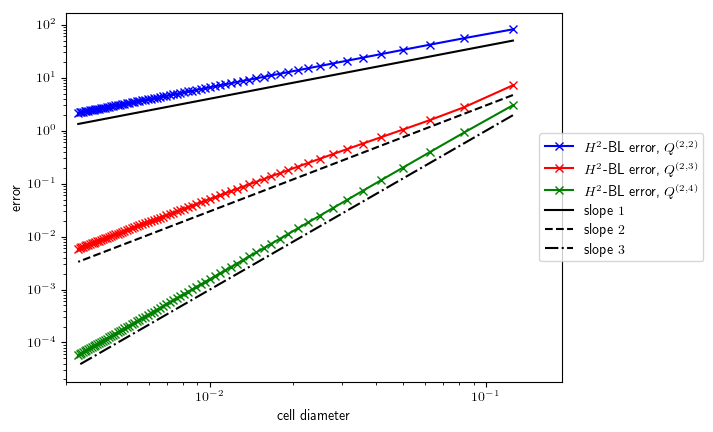
\includegraphics[width=4in]{Pictures/oned-cdr-2-h2-errors.png}

        \caption{Convergence rates for the \(p\)-refinement scheme of the second
        derivative on the boundary.}
    \end{figure}
\end{frame}

\section{\(p\)-refinement in 2D}
    \begin{frame}
        \frametitle{Extension to 2D at Mesh Knots}
        With periodic boundary conditions we can use Fourier mode interpolants
        as trial functions:
        \begin{equation*}
            u^h(x, y) = \sum_{k = 0}^{N - 1} F_k(x) \hat{u}^h_k(y) :
            F_k(x) \in V^{\Delta x}([0, 1]),
            \hat{u}^h(y) \in V^{\Delta y}([0, L]).
        \end{equation*}
        \pause
        \begin{equation*}
            \int_0^L
            \hat{u}^h_{k, y} \bar{\phi}_y
            + b_1 \hat{u}_{k, y} \bar{\phi}
            + \dfrac{\lambda_{A, k}}{\lambda_{M, k}}
            \hat{u}^h_k \bar{\phi} dy
            =
            \int_0^L
            \left(
            \int_0^1
            \dfrac{f(x, y) F_k(x)}{\lambda_{M, k}} dx
            \right)
            \bar{\phi} dy,
            \forall \phi(y) \in V^{\Delta y}.
        \end{equation*}
        Here \(\lambda_{M,k}\) and \(\lambda_{A,k}\) are eigenvalues of the
        (circulant) 1D mass and stiffness matrices.
        \pause
        \begin{center}
            The 1D result applies to each \(\hat{u}^h_k(y)\), implying normal
            derivative superconvergence at mesh knots.
        \end{center}
    \end{frame}

\begin{frame}
    \frametitle{Numerical Results}
    Manufactured solution with \(\vec{b} = (1, 1)\) and \(c = 2\):
    \begin{equation*}
        u(x, y) = (y^3 + \exp(-y^2) + \sin(4.5 y^2) + \sin(20 y)) (20 \cos(4 \pi x)
        + 0.1 \sin(20 \pi x) - 80 \sin(6 \pi x))
    \end{equation*}
    \pause
    \(H^1{\hyphen}B\) error defined as
    \begin{equation*}
        \max_{i, j}
        \left|
        (\nabla u^h \cdot \vec{n} -
        \nabla u \cdot \vec{n})(\delta_i, \delta_j)
        : (\delta_i, \delta_j) \in \partial \Omega^h
        \right|
    \end{equation*}
    and \(H^2{\hyphen}B\) error defined as
    \begin{equation*}
        \max_{i, j}
        \left|
        (\vec{n}^T \Delta u^h \cdot \vec{n} -
        \vec{n}^T \Delta u \cdot \vec{n})(\delta_i, \delta_j)
        : (\delta_i, \delta_j) \in \partial \Omega^h
        \right|.
    \end{equation*}
\end{frame}

\begin{frame}
    \frametitle{Numerical Results}
    \begin{figure}
        \centering
        Elimination of nonnormal \(p\)-refinement:
        \begin{tikzpicture}[scale=1.5]
    %% leftmost pair
    % cubic square
    \draw[-, thick] (-1.0, 0.0) -- (-1.0, 1.0);
    \draw[-, thick] (0.0, 0.0) -- (0.0, 1.0);
    \draw[-, thick] (-1.0, 0.0) -- (0.0, 0.0);
    \draw[-, thick] (-1.0, 1.0) -- (0.0, 1.0);

    % linear square
    \draw[-, thick] (-1.0, -1.0) -- (-1.0, 0.0);
    \draw[-, thick] (0.0, -1.0) -- (0.0, 0.0);
    \draw[-, thick] (-1.0, -1.0) -- (0.0, -1.0);
    \draw[-, thick] (-1.0, 0.0) -- (0.0, 0.0);

    % cubic support points
    \foreach \x in {0,...,4}
    \foreach \y in {0,...,4}
        \draw (0.25*\x - 1.0, 0.25*\y) node[cross] {};

    % linear support points
    \foreach \x in {0,...,1}
    \foreach \y in {0,...,1}
        \draw (\x - 1.0, \y - 1.0) circle (2pt);

    %% second pair
    % cubic square
    \draw[-, thick] (0.0, 0.0) -- (0.0, 1.0);
    \draw[-, thick] (1.0, 0.0) -- (1.0, 1.0);
    \draw[-, thick] (0.0, 0.0) -- (1.0, 0.0);
    \draw[-, thick] (0.0, 1.0) -- (1.0, 1.0);

    % linear square
    \draw[-, thick] (0.0, -1.0) -- (0.0, 0.0);
    \draw[-, thick] (1.0, -1.0) -- (1.0, 0.0);
    \draw[-, thick] (0.0, -1.0) -- (1.0, -1.0);
    \draw[-, thick] (0.0, 0.0) -- (1.0, 0.0);

    % cubic support points
    \foreach \x in {0,...,4}
    \foreach \y in {0,...,4}
        \draw (0.25*\x, 0.25*\y) node[cross] {};

    % linear support points
    \foreach \x in {0,...,1}
    \foreach \y in {0,...,1}
        \draw (\x, \y - 1.0) circle (2pt);

    \draw[->, thick] (1.5, 0.0) -- (2.5, 0.0);

    % cubic square
    \draw[-, thick] (3.0, 0.0) -- (3.0, 1.0);
    \draw[-, thick] (4.0, 0.0) -- (4.0, 1.0);
    \draw[-, thick] (3.0, 0.0) -- (4.0, 0.0);
    \draw[-, thick] (3.0, 1.0) -- (4.0, 1.0);

    % linear square
    \draw[-, thick] (3.0, -1.0) -- (3.0, 0.0);
    \draw[-, thick] (4.0, -1.0) -- (4.0, 0.0);
    \draw[-, thick] (3.0, -1.0) -- (4.0, -1.0);
    \draw[-, thick] (3.0, 0.0)  -- (4.0, 0.0);

    % cubic support points
    \foreach \x in {0,...,1}
    \foreach \y in {0,...,4}
        \draw (3.0 + \x, 0.25*\y) node[cross] {};

    % linear support points
    \foreach \x in {0,...,1}
    \foreach \y in {0,...,1}
        \draw (3.0 + \x, \y - 1.0) circle (2pt);

    %% rightmost pair
    % cubic square
    \draw[-, thick] (4.0, 0.0) -- (4.0, 1.0);
    \draw[-, thick] (5.0, 0.0) -- (5.0, 1.0);
    \draw[-, thick] (4.0, 0.0) -- (5.0, 0.0);
    \draw[-, thick] (4.0, 1.0) -- (5.0, 1.0);

    % linear square
    \draw[-, thick] (4.0, -1.0) -- (4.0, 0.0);
    \draw[-, thick] (5.0, -1.0) -- (5.0, 0.0);
    \draw[-, thick] (4.0, -1.0) -- (5.0, -1.0);
    \draw[-, thick] (4.0, 0.0)  -- (5.0, 0.0);

    % cubic support points
    \foreach \x in {0,...,1}
    \foreach \y in {0,...,4}
        \draw (4.0 + \x, 0.25*\y) node[cross] {};

    % linear support points
    \foreach \x in {0,...,1}
    \foreach \y in {0,...,1}
        \draw (4.0 + \x, \y - 1.0) circle (2pt);
\end{tikzpicture}

        \caption{Depiction of normal \(p\)-refinement scheme, with elimination
        of extra DoFs. Linear DoFs are circles, quartic are crosses.}
    \end{figure}
\end{frame}

\begin{frame}
    \frametitle{Numerical Results}
    \begin{figure}
        \centering
        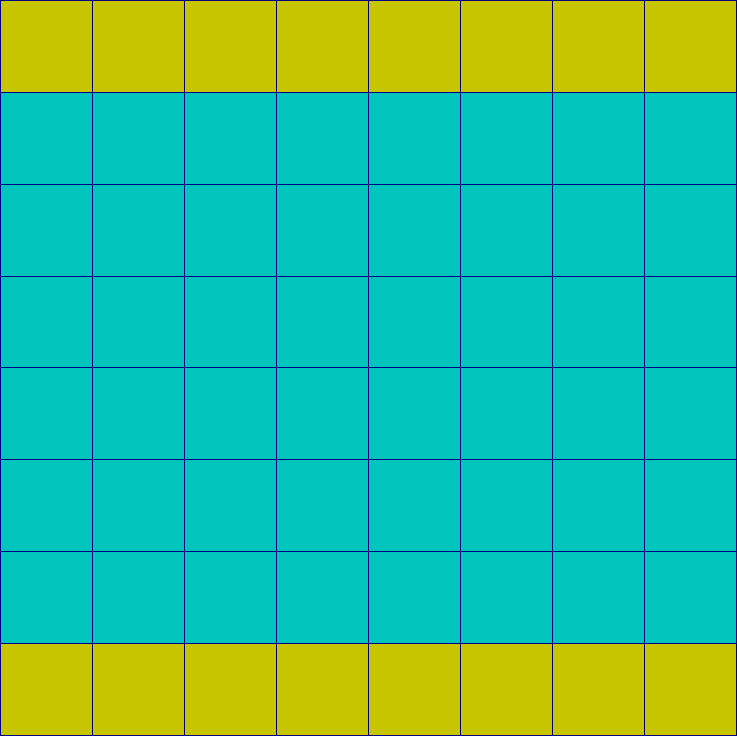
\includegraphics[width=2.5in]{Pictures/square-periodic-grid.png}

        \caption{Depiction of the square grid with bulk cells in cyan and
        \(p\)-refined cells in yellow.}
    \end{figure}
\end{frame}

\begin{frame}
    \frametitle{Numerical Results}
    \begin{figure}
        \centering
        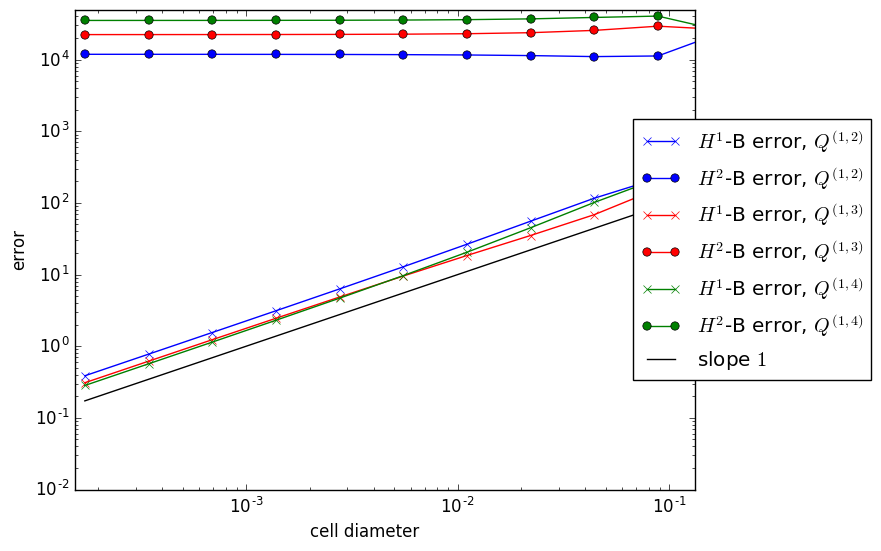
\includegraphics[width=3in]{Pictures/periodic-dont-eliminate-nonnormal-convergence.png}

        \caption{Convergence rates with anisotropic \(p\)-refinement. We do not
        recover any higher order accurate derivatives.}
    \end{figure}
\end{frame}

\begin{frame}
    \frametitle{Numerical Results}
    \begin{figure}
        \centering

        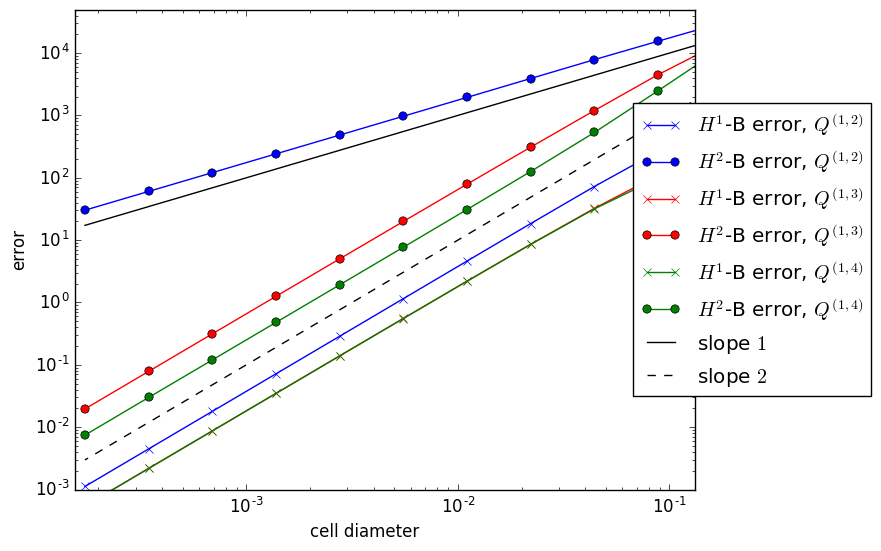
\includegraphics[width=3in]{Pictures/periodic-nonnormal-convergence.png}

        \caption{Convergence rates with isotropic \(p\)-refinement. The 1D
        theory applies at the knots.}
    \end{figure}
\end{frame}

\begin{frame}
    \frametitle{Numerical Results}
    \begin{figure}
        \centering

        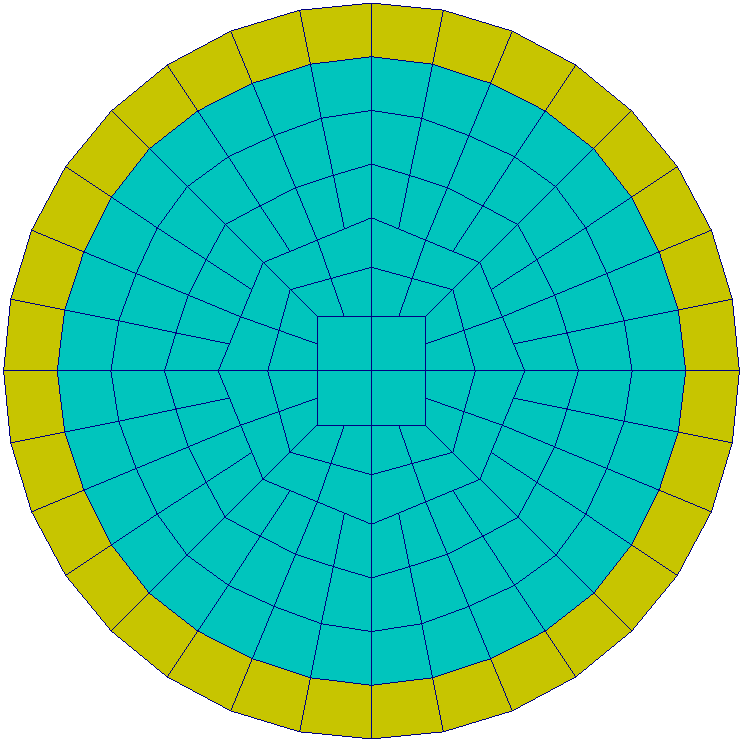
\includegraphics[width=2.5in]{Pictures/circular-grid.png}
        \caption{A circular grid with a geometry described near the boundary in
        polar coordinates, in the middle with Cartesian coordinates, and a
        transfinite interpolation in-between.}
    \end{figure}
\end{frame}

\begin{frame}
    \frametitle{Numerical Results}
    \begin{figure}
        \centering

        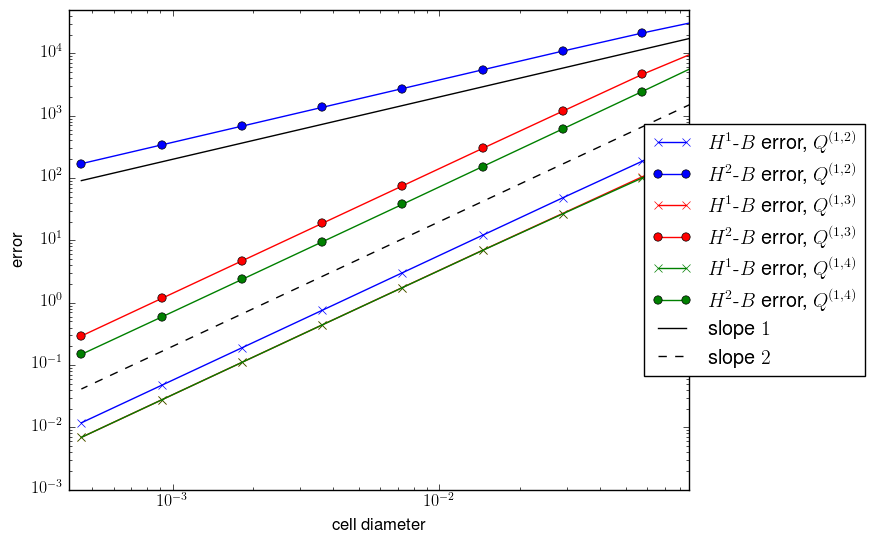
\includegraphics[width=3in]{Pictures/circle-nonnormal-convergence.png}
        \caption{Rates of convergence for the circular grid.}
    \end{figure}
\end{frame}

\section{Summary}
\begin{frame}
    \frametitle{Summary and Outlook}
    \begin{itemize}
        \item \(p\)-refinement error estimates involve a coupling term and a
              local term
        \item We can achieve higher-order derivative approximation at isolated
              points
        \item Future work: escape the Fourier framework, higher-order bulk
              elements, better tools for describing arbitrary geometries
    \end{itemize}

    \vspace{0.5in}
    \begin{center}
        \textcolor{Carolinablue}{\Huge Thank You!}
    \end{center}
\end{frame}

\end{document}
